
\chapter{Introduction}

This document discusses \emph{routeMatching} in the \emph{OpenRideShare} Application.

OpenRideShare (henceforth abbreviated \emph{"ORS"}) is an application that provides \emph{RideSharingServices}.
The OpenRideShare Software is largely based on the codebase a predecessor named "OpenRide". OpenRide was provided by 
the \emph{FOKUS, Fraunhofer Institute f\"ur offene Kommunikationssysteme}. OpenRide went OpenSource in 2011, but
was not developed further by FOKUS. So, the code was picked up by a bunch of enthusiastic enthusiasts and developed 
further, now under the label \emph{"OpenRideShare"}. 

\section{Rideshareing and Dynamic Rideshareing}
\index{Rideshareing}

Suppose that Janet wants to drive from  Douglas to  Ramsay (both towns on the Isle of Man in the Irish Sea),
and that Janet has some empty seats in her car, which she would like to share with someone else travelling  that direction.
Next, suppose that at the same time Bob wants to travel from Baldrine (which is close to Douglas) to Port Lewaigue 
(which is close tho Ramsay).
Picking up Bob at Baldrine and dropping him at Port Lewaigue would add only some small detour to Janet's route. 
If this detour is within a maximum detour that Janet is willing to go, than it makes sense for Janet  
and  Bob to travel together, i.e share a ride, and maybe a portion of the ride's costs.

OpenRideShare offers the capabilitiy to bring drivers (like Janet) and riders (like Bob) together.
Via a mobile interface it is also possible for drivers to find matching requests in "real time", while 
the driver is already on the road. This is sometimes called \emph{"Dynamic Rideshareing"}.
\index{Dynamic Rideshareing}

\section{Route Matching}
\index{Route Matching}
\emph{Route Matching} is the act of bringing together matching offers and requests. 
This is the core functionality of OpenRideShare (and, of course any dynamic ridesharing application)
Technically, route matching comprises either one of the following two actions:
\label{routeMatchingIntroduction}
\begin{enumerate}
\item{When a new offer is created, search for matching requests }
\item{When a new request is created, search for matching offers}
\end{enumerate}

As seen in the previous short example with Janet and Bob, the places where Bob has to be picked up and dropped are
close to Janet's route, but not exactly on it, which forces Janet to slightly alter her route, and go a small 
detour. Finding matches thus comprises calculating and testing alternative routes, which is a notoriously costly operation.
Thus, the ORS's route matching algoritms aim at doing a preselection of rides that limits the actual cases
where an altered route has to be calculated to as few as possible matches.
The rest of this document is mainly about how this is done.


\section{Offers, Requests and Route Matching in more Detail}

In this section we discuss the process of creating offers and request, the
creation of routes, and route matching from a highlevel perspective.

\section{Creating an Offer}
\index{Offer}
Before starting her journey, Janet enters some data about the journey into the ORS.
These data mainly comprise:

\begin{itemize}
\item{The place where the journey starts (In our example: \emph{"Douglas"})}
\item{The place where the journey ends (In our example: \emph{"Ramsay"})}
\item{Optionally some additional points she wants to visit on her way (called \emph{"waypoints"}).
      For simplicity, we do not have waypoints in our example.
      }
\item{Date and time when Janet wants to start}
\item{ A \emph{"maximum detour"} parameter, giving the maximal detour that Janet is willing
       to go when picking up coriders.	
      }
\item{The Number of free seats Janet wants to offer}
\item{Optionally a number of criteria such as gender, smoker/nonsmoker, etc 
      which can be used to filter potential riders
     }
\end{itemize}

\section{The Route}
\label{theRoute}
\index{Route}

Given these data, ORS invokes a \emph{Routing engine} to calculate a \emph{route} for
Janet.  Technically, the route is an ordered list of so called  \emph{Routepoints}, 
with each Routepoint containing the following data:
\index{Routepoint}
\begin{itemize}
\item{Spatial Coordinates in polar longitude/latitude form
              and in addition in some suitable local carthesian coordinate system 
              for speedy calculation of distances)}
\item{A timestamp describing when Janet passes this point}
\item{A reference to Janet's offer}
\end{itemize}

\begin{figure}[t]
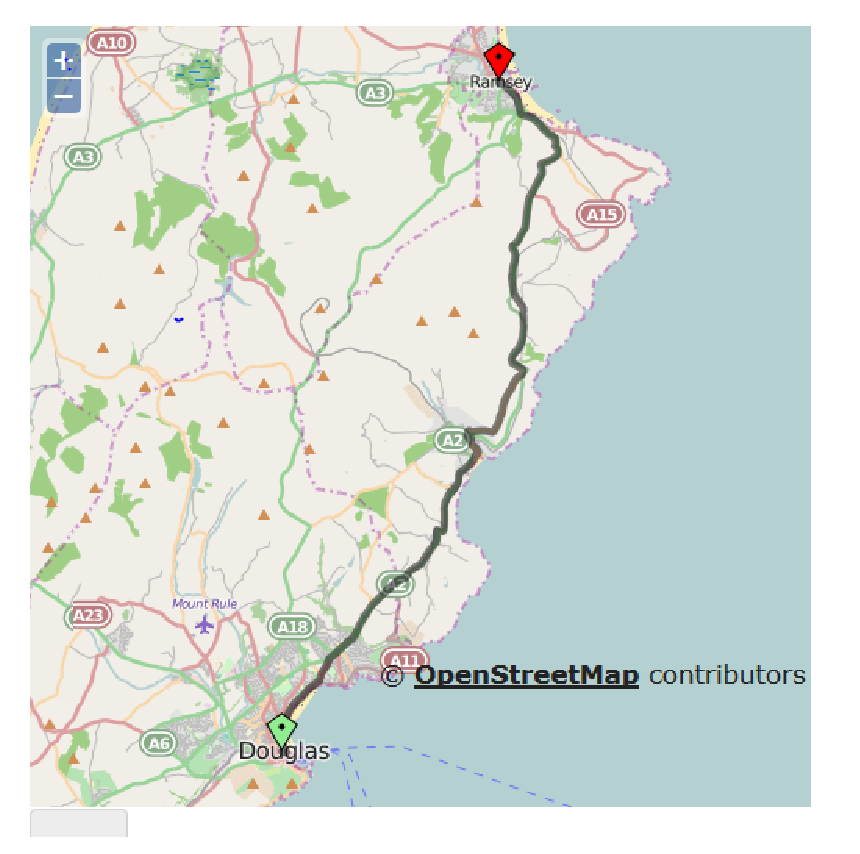
\includegraphics[scale=0.5]{images/maps/01-OSM-DouglasToRamsay.eps}
\caption{Janet's route from Douglas to Ramsay as calculated by ORS}
\label{pic:janetRoute}
\end{figure}


Figure~\ref{pic:janetRoute} shows Janet's route from Douglas to Ramsay, as calculated by ORS.

\section{Creating a Request}
\index{Request}
Now Bob wants to travel from Baldrine to Port Lewaigue, which is roughly on Janet's way. 
Not wanting to drive with his own car, Bob takes his chances with OpenRideShare and creates a 
\emph{request} in ORS. 
To create a request, Bob has to enter the following data:

\begin{description}


\item[startpt]{The place where the journey starts (In our example: \emph{"Baldrine"})}
\item[endpt]{The place where the journey ends (In our example: \emph{Port Lewaigue})}

\item[startTimeEarliest]{A timestamp describing the earliest time when Bob wants to start.}
\item[startTimeLatest]{A timestamp describing the latest time when Bob wants to start.}
\item[criteria]{Optionally: a number of criteria such as gender, smoker/nonsmoker, etc 
      which can be used to filter potential drivers.  	
     }
\end{description}

\section{Route Matching in more Detail}
\index{Route Matching}
The route matching step is applied immeadiately after creating an offer or request.
We discuss route matching for a newly created offer briefly in  \ref{searchForRiderShort},
and extensively in section \ref{searchForRiders}.
Route matching for a newly created request is discussed briefly in  \ref{searchForRiderShort},
and extensively in section \ref{searchForDrivers}.


\subsection{Finding matching Requests for a given Offer}
\index{Offer!finding matching requests for given offer}
\index{Request!finding matching requests for given offer}
\label{searchForRiderShort}

As seen in section \ref{theRoute}, along with an offer a route gets created.
Next, along that route a corridor of width \emph{detour} is searched for requests that 
have either start or endpoint in that corridor.

Here \emph{corridor}, means the places that have \emph{direct distance} \emph{detour} from the route, 
not \emph{road distance}. While for calculating the road distance expensive routing functionality has 
to be used, direct distances (aka "as the crow flies") can be calculated with little effort and 
provide a good upper bound for road distances. 
\index{Corridor}
If a request is found that has both start and endpoint in that corridor, and with
the startpoint matching the temporal bounds, then the associated request is
preselected for final filtering.

In the final filtering step, first the "optional parameters" (smoker, gender,...) 
are tested. For all request passing this filter, finally an exact route containing 
the start and endpoint of the request is calculated. 
If this route does not exceed the original route by more then detour, the request
is considered to be successfully matched.
It then gets displayed to the rider and driver in the frontend for approval.

Figure \ref{pic:bobRoute} shows Janet's altered route with places to pick up and
drop Bob marked by the small round icons showing an arrow and a suitcae. 

Janet's new route now includes small detours to pick up Bob at 
Baldrine (see figure \label{pic:bobRouteDetourPickup} for closeup)
and dropping Bob at Port Lewaigue (see figure \ref{pic:bobRouteDetourDrop} for closeup)
\index{Detour}

\begin{figure}[t]
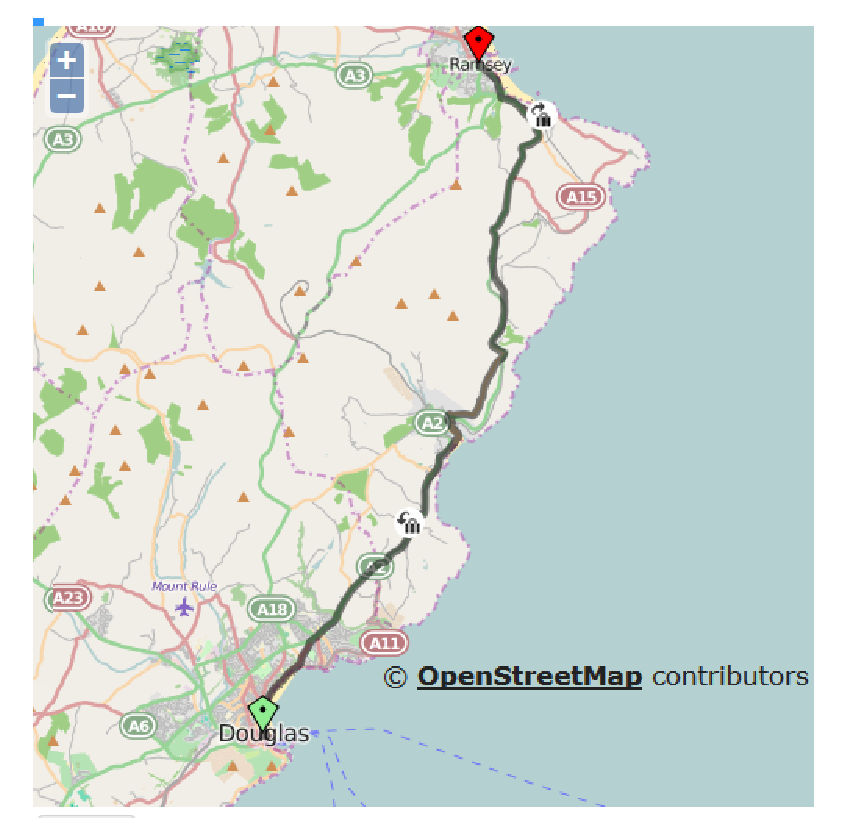
\includegraphics[scale=0.5]{images/maps/02-OSM-with-Rider.eps}
\caption{Janet's route from Douglas to Ramsay, including small detours to pick up Bob
        ad Baldrine and drop him at Port Lewaigue.}
\label{pic:bobRoute}
\end{figure}


\begin{figure}[h]
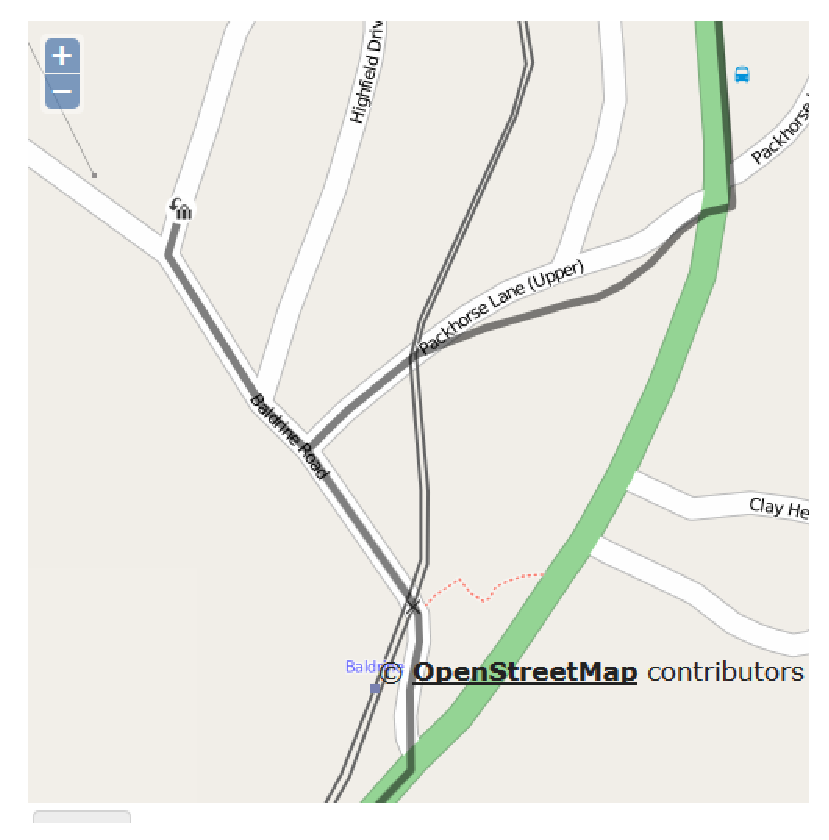
\includegraphics[scale=0.25]{images/maps/03-OSM-Pickup-Baldrine.eps}
\caption{Janet's new route in detail, including the detour from main road A2 (green) to pick up Bob at Baldrine}
\label{pic:bobRouteDetourPickup}
\end{figure}

\begin{figure}[h]
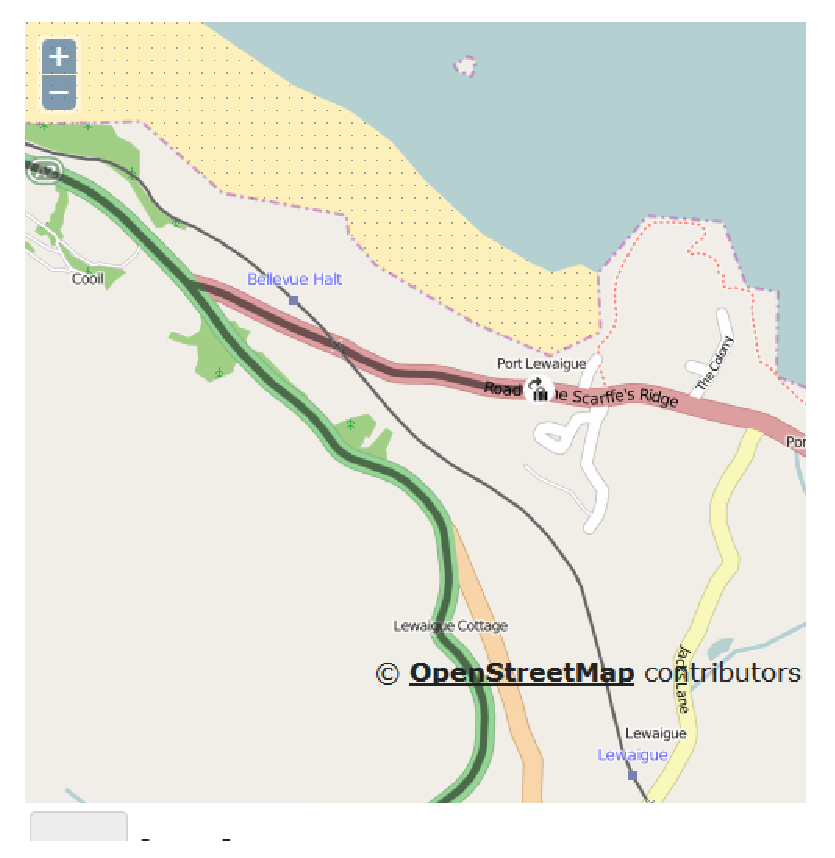
\includegraphics[scale=0.25]{images/maps/04-OSM-Drop-Lewaigue.eps}
\caption{Janet's new route in detail, including the detour from main road A2 to drop Bob at Port Lewaigue }
\label{pic:bobRouteDetourDrop}
\end{figure}


\subsection{Finding matching Offers for a given Request}
\label{searchForDriverShort}
\index{Offer!finding matching offers for given request}
\index{Request!finding matching offers for given request}
Finding matching offers for a given request comprises the following steps:

\begin{enumerate}
\item{ For the request's starting point, determine all offers that have 
       routepoints coming within distance "detour" to the starting point 
       and match the temporal bounds.}
\item{Determine all offers that come within range of "detour" to the drive's endpoint.}
\end{enumerate}
\index{Detour}
The intersection set of the requests in (1) and (2) is determined, and the offers in the intersection sets
are filtered analogously to the processing at the final step of \ref{searchForRiderShort}:
\index{Filtering Criteria (cheap)}
First, the "cheap" filtering criteria (smoker, gender,..) are applied, and finally for the remaining
request, the detour-route is calculated and it is checked if the detour is in the detour defined 
by the driver.

All offers that pass the final test are then presented to driver and rider for approval.
\index{Approval}
